\chapter{静磁场}
\section{毕奥-萨伐尔定律}
\subsection{毕奥-萨伐尔定律}
电流元$I\mathbf{d}\vec{l}$在空间任一点P处所激发磁场的磁感应强度为
$$\mathbf{d}\vec{B}=\frac{\mu_0}{4\pi}\frac{I\mathbf{d}\vec{l}\times\vec{e_r}}{r^2}$$

电流元：用矢量$I\mathbf{d}\vec{l}$表示。其中$\mathbf{d}\vec{l}$表示在载流导线上（沿电流方向）所取的线元，$I$为导线中的电流，电流元的方向规定为电流沿线元的流向。

$\mu_0=4\pi\times10^{-7}T\cdot m/A$，称为真空磁导率。

$\vec{e_r}$是从电流元所在处到场点$P$的位矢。

\subsection{应用示例}
\subsubsection{载流直导线}
对于长为$L$的载流直导线，距离直导线为$a$的$P$点的磁感应强度：
$$B=\frac{\mu_0 I}{4\pi a}(\sin\beta_2-\sin\beta_1)$$
\begin{figure}[h]
	\centering
	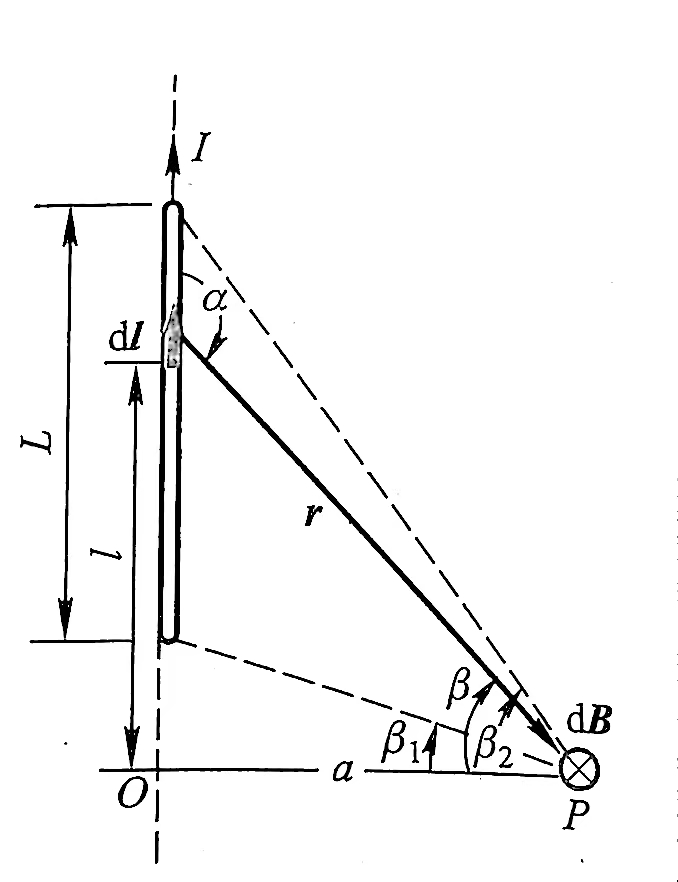
\includegraphics[width=0.3\textwidth]{images/8.3 载流直导线.jpg}
	\caption{载流直导线附近磁场的计算}
\end{figure}

对于无限长载流直导线，取$\beta_1=-\pi/2$，$\beta_2=\pi/2$，得：
$$B=\frac{\mu_0 I}{2\pi a}$$

\subsubsection{载流圆线圈的轴线}
$$B=\frac{\mu_0}{2\pi}\frac{IS}{(R^2+x^2)^{3/2}}$$
\begin{figure}[h]
	\centering
	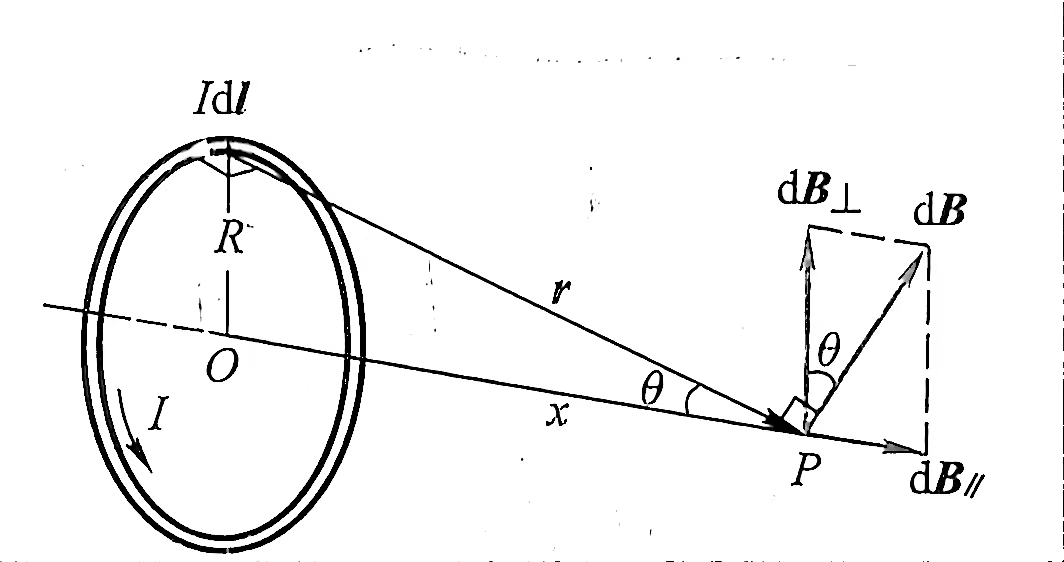
\includegraphics[width=0.5\textwidth]{images/8.3 圆电流轴线.jpg}
	\caption{圆电流轴线上磁场的计算}
\end{figure}

在圆心$x=0$处，$B_0=\frac{\mu_0I}{2R}$

当$x\gg R$时，$B=\frac{\mu_0IS}{2\pi x^3}$

引入磁矩$\vec{m}=IS\vec{e_n}$（若线圈有$N$匝，则磁场加强$N$倍，$\vec{m}=NIS\vec{e_n}$），其中$\vec{e_n}$表示线圈平面法线方向的单位矢量（由线圈中电流流向按右手螺旋定则确定）。则：
$$\vec{B}=\frac{\mu_0\vec{m}}{2\pi x^3}$$
\begin{figure}[h]
	\centering
	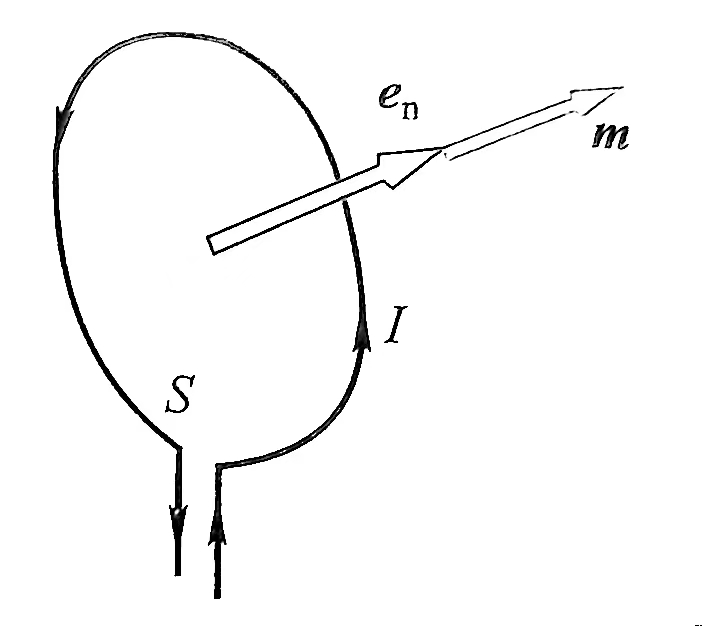
\includegraphics[width=0.3\textwidth]{images/8.3 磁矩.jpg}
	\caption{磁矩的方向}
\end{figure}

\subsubsection{载流直螺管内部}
\begin{figure}[h]
	\centering
	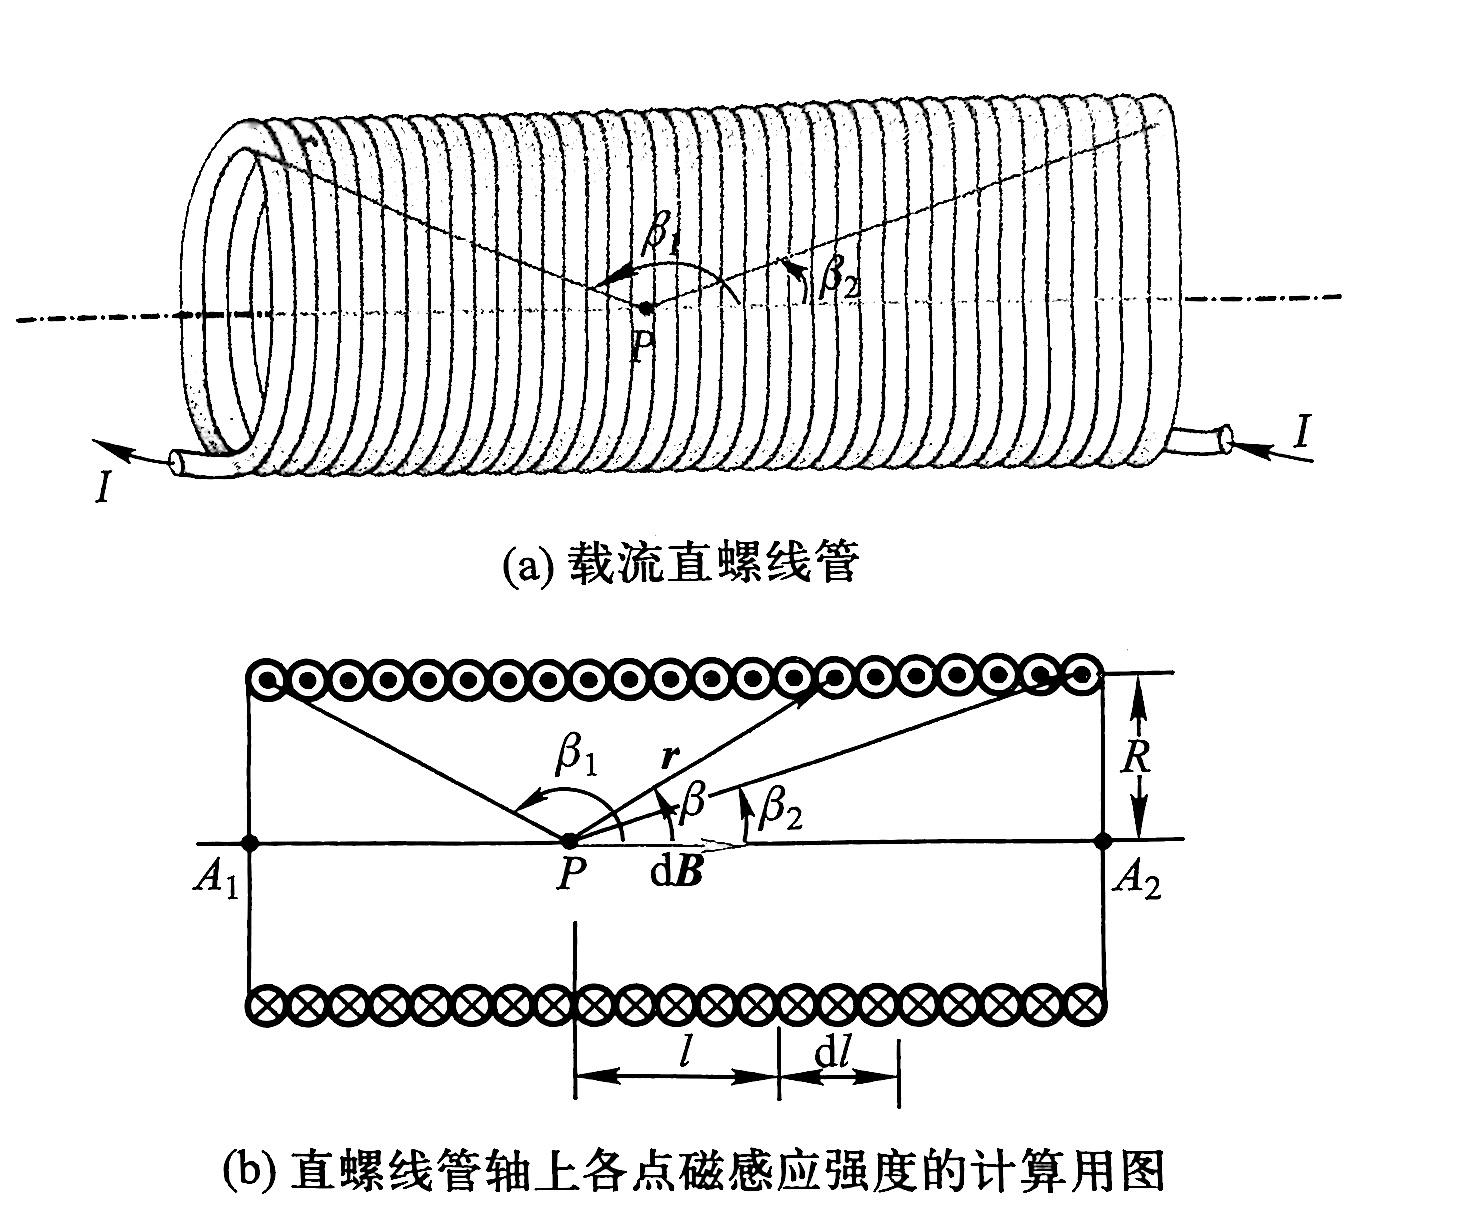
\includegraphics[width=0.5\textwidth]{images/8.3 直螺线管内部.jpg}
	\caption{直螺线管内部磁场的计算}
\end{figure}
螺线管半径为$R$，电流为$I$，每单位长度有线圈$n$匝：
$$B=\frac{\mu_0}{2}nI(\cos\beta_2-\cos\beta_1)$$

无限长螺线管，亦即螺线管的长度$\gg$其直径时：
$$B=\mu_0 nI$$

长螺线管的端点：
$$B=\frac{1}{2}\mu_0 nI$$

\subsection{运动电荷的磁场}
每一个以速度$v$运动的电荷所激发磁场的磁感应强度$B_q$为：
$$B_q=\frac{\mu_0}{4\pi}\frac{q\vec{v}\times\vec{e_r}}{r^2}$$